\documentclass{article}

\usepackage{graphicx}
\usepackage{hyperref}
\usepackage{amssymb}

\title{Yelp and Crime}  % TODO
\author{Kenneth Lin, Sid Naik, Tom McCormick}
\date{\today}

\renewcommand{\labelitemi}{\checkmark}

\begin{document}
\maketitle

\section{Problem Statement and Background}

For our CS 194 final project, we decided to investigate the potential
relationship between the City of San Francisco public safety data set and
the data set provided by the Yelp API. With the recent civil unrest both
inside and outside of the United States, and more recently, right here in
Berkeley, we thought that it would be interesting to look into the factors
that promote crime. One of our team members (Kenneth Lin) had also been
robbed recently, so the problem is one that is dear to our hearts. Perhaps
the most well-known correlation with crime rate is the income level of a
neighborhood -- the lower the income level, the higher the crime rate
\cite[p.93-94]{levitt-the-changing-relationship}. However, we wanted to
show something more interesting. In particular, Yelp restaurants, in our
experience, often reflect the wealth and well-being of its surrounding
neighborhood -- the presence of many highly rated restaurants, we believed,
reflect the optimism in the economy of a neighborhood, as well as the
wealth and ``goodness'' of that neighborhood. Therefore, we had conjectured
that crime would negatively impact restaurant ratings, or that low
restaurant ratings would be correlated with areas of high crime. We worked
to show this throughout our project.

% At first, we explored each data set individually to discover general
% patterns in the data set. After that, we delved into our main problem. We
% are interested in the relationship (if any) between the quality of
% restaurants and the frequency and severity of crime. In particular, we
% wanted to know

In particular, we wanted to know

\begin{itemize}
\item the effect of crime on restaurant ratings (or vice versa)
\item the distribution of crime vs. the distribution of ratings
\end{itemize}

We had also wanted to predict crime density / severity using restaurant
ratings or vice versa, but along the way we ran into issues of determining
or implying causation in any of the methods we used. By using one to
predict the other and trying to draw useful conclusions from this, we run
the risk of assuming causation without definitive proof. There are many
other problems that may arise as a result of this, which will be discussed
in the \textbf{\nameref{sec:lessons-learned}} section.

\subsection{City of San Francisco Public Safety Data Set}

The City of San Francisco public safety data set is a record, written by the
San Francisco Police Department, of incoming incident reports, either via
phone call, in person, or otherwise. The incidents are reported via the
SFPD CABLE crime incident reporting system. The incidents are reported over
the course of more than 11 years, from 1/1/2003 to present. Incidents are
recorded when a police report is filled out during or after a crime
incident. Crimes range from aggravated assault to vandalism to death
reports.

A sample of records in the data set looks like the following:

\begin{center}
  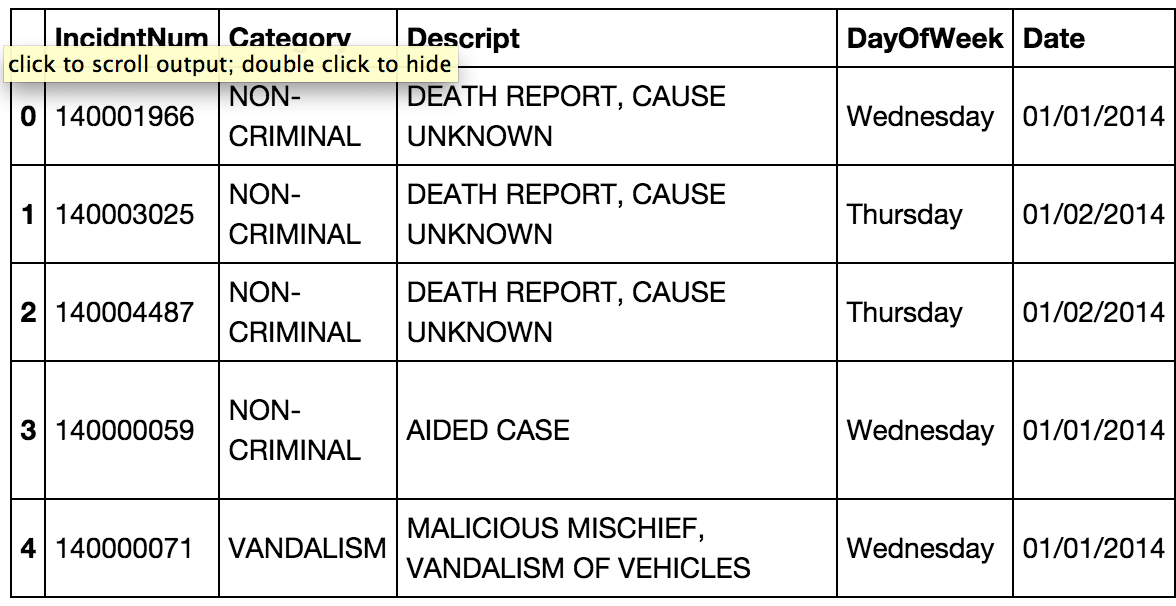
\includegraphics[scale=0.5]{sf_city_sample_1.png} \\
  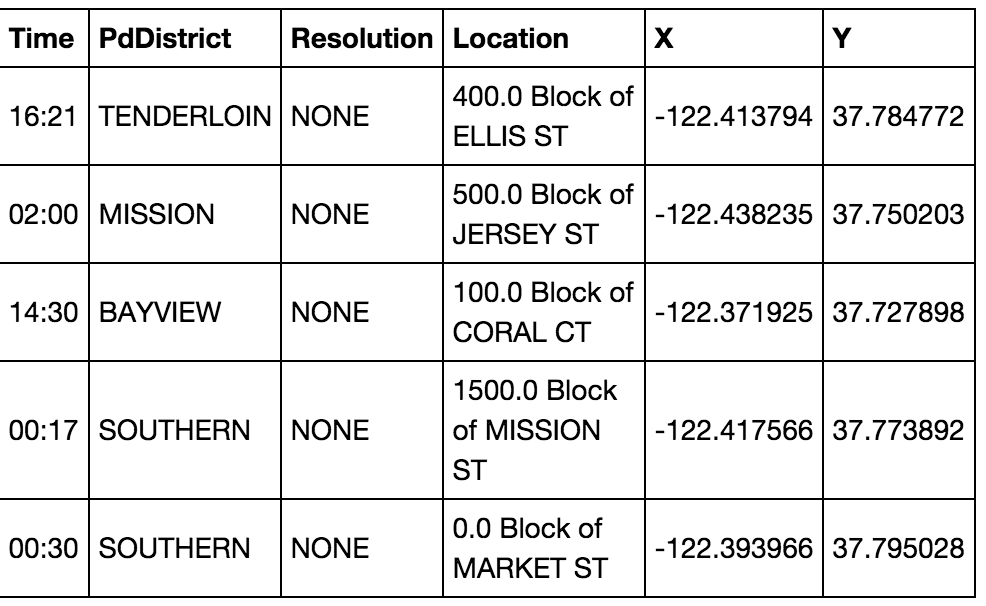
\includegraphics[scale=0.5]{sf_city_sample_2.png} \\
  Figure 1: Sample of San Francisco crime data set
\end{center}

The majority of the fields are self-explanatory. However, there are a few
things to note:
\begin{enumerate}
\item Category and descript are both categories, but category is more
  general. There are only 36 different ``Categories'' while there are 499
  different ``Descript''s in the year of 2014.
\item Resolution, though none are shown in the sample above, denote whether
  any action was taken and what that action was.
\item X denotes longitude, while Y denote latitude.
\end{enumerate}

A more detailed analysis is in the attached \texttt{analysis.ipynb}.

\subsection{Yelp Data Set}

Yelp.com is a platform which publishes crowd-sourced reviews about local
businesses. On Yelp, customers who have used the services of local
businesses may write reviews of these businesses and provide ratings of
their satisfaction. Reviewers may select from between 1 to 5 stars for each
review they make, and a business's average rating is the average of the
ratings of each of the reviews it has received. Yelp supplies a platform
for all kinds of local businesses ranging from restaurants to barbers to
museums; however, for the purpose of our research, we will look primarily
at restaurants as they are a very large majority of the reviews on Yelp.

There are two primary ways to access the data on Yelp. First, we can
utilize the search / business API
(\url{http://www.yelp.com/developers/documentation}). The API provides a
way to search for local businesses matching a particular key term
(``restaurants'', for example) near a geographical location, and get all
the rating / review information about that restaurant. The API further
allows us to narrow the search to only the geographically closest
restaurants (not ranked by rating). This gives us a way to link the
geographical location of crime incidents to the types of restaurants near
that incident.

The other way of accessing Yelp data is through the academic data set
(\url{https://www.yelp.com/academic_dataset}). The Yelp academic data set
provides all the data and associated reviews of the 250 closest businesses
to each of 30 universities, including UC Berkeley. Although not a random
sample of all businesses on Yelp, the academic data set provides a much
better estimate of all businesses in the Yelp data set population.

-- basic analysis

\section{Methods}

\subsection{Data Fetching}

The bulk of our work was done in trying to get data from Yelp. As
mentioned, there were two main ways that Yelp provides to access data, and
those are the API and the academic data set.

To access the Yelp API, Yelp provided sample Python code
(\url{https://github.com/Yelp/yelp-api/tree/master/v2/python}). However, as
we found out, the sample code was buggy -- not only did the code fail on
certain calls, it even failed on the default call when the search term was
``dinner'' and the location was ``San Francisco, CA''. We contacted Yelp
API support about this issue, but it seemed that the API wasn't
well-maintained, and Yelp engineers didn't have time to update or fix the
sample code. Therefore, we decided to fix the bug ourselves.

After much investigation, we figured out that whereas Python's
\texttt{urllib} library encoded spaces into ``+'' characters, Yelp's
server-side authentication expected the OAuth-signed URLs to use ``\%20''
as the proper encoding for space. In this context (the query arguments in a
URL), both should be valid, but Yelp's authenticator only expected the
latter. After figuring this out, we let the Yelp engineers know of the bug,
and were able to begin building a temporary work-around to fetch our data.

We also encountered other problems in data fetching. In addition to the
bugs in the API, there were rate limiting and quantity limiting issues as
well. In particular, we could only access 20 results at a time, and a
maximum of 40 total results for searches that sorted the results by only
distance or rating. This limited the ways in which we could obtain and
analyze Yelp data.
% TODO something about some ideas we had
Further, we weren't able to get as much data as we needed (because of
Yelp's rate limiting). However, it was still possible to search for the
closest restaurants near any location specified by longitude and
latitude. As a result, we decided to search for the 20 closest restaurants
near each crime and look at the characteristics of this set of restaurants.

In the end, we were able to build a fault-tolerant work-around to Yelp's
broken authentication system. We queried Yelp's API for the 20 closest
restaurants near each crime in the City of San Francisco crime data set for
a total of 12,000 crimes (9704 unique incidents due to multiple criminal
offenses per incident). These results were stored in our MongoDB instance
that we installed on our EC2 server.

\subsection{Visualization}

% TODO
% TODO do yelp rating map

\subsection{Looking for Correlations}

\subsection{Accounting for Population Density}

-- tract difficulties, calculating tract centers

\subsection{Predicting Crimes}

% TODO more subsections

\section{Tools}

\begin{itemize}
\item pandas -- Pandas was our primary means of manipulating data sets. We
  used Pandas in our data fetching, data cleaning, and data analysis
  process.
\item MongoDB -- We installed MongoDB on the EC2 server and used it
  primarily for storing Yelp data. MongoDB was a great choice because the
  document-based nature of MongoDB was perfect for storing all the JSON
  documents we received from the Yelp API. In addition, we weren't sure
  what kind of data we needed to store when we first began fetching data,
  so using Mongo allowed us to easily keep all of the data in case we
  needed more than what we had thought.
\item pyMongo -- pyMongo was our choice Python interface to MongoDB.
\item numpy -- NumPy was used in conjunction with both Pandas and SciPy.
\item scipy -- We used SciPy mostly for its large library of statistical
  methods (t-tests, etc.).
\item D3.js -- We used D3 in conjunction with other frameworks when
  visualizing the data.
\item Google Maps API -- The Google Maps API provided a base for many of
  the location-based visualizations we needed to create. In addition, the
  Google Maps API also had a heatmap plugin, which we tried in addition to
  heatmap.js.
\item heatmap.js -- We primarily used heatmap.js for our heatmap
  visualizations.
\end{itemize}

\section{Results}

\subsection{Putting it together}

-- distribution
-- ratings

-- CONCLUSIONS??!?

-- map visualization problems
---- yelp data biased to near crime
---- not enough data on all of san francisco to create proper viz

-- condition tests in certain neighborhoods

\section{Lessons Learned}
\label{sec:lessons-learned}

-- Yelp API shit; no one uses
-- data cleaning hard
-- causation and correlation
-- problem statement
-- problems with the data (not sure where it's from)
-- don't draw conclusions before the results are out

\bibliographystyle{IEEEtran}
\bibliography{writeup-bibliography}

\end{document}
